\documentclass[10pt]{article}
\usepackage[polish]{babel}
\usepackage[utf8]{inputenc}
\usepackage[T1]{fontenc}
\usepackage{graphicx}
\usepackage[export]{adjustbox}
\graphicspath{ {./images/} }
\usepackage{amsmath}
\usepackage{amsfonts}
\usepackage{amssymb}
\usepackage[version=4]{mhchem}
\usepackage{stmaryrd}

\title{ARKUSZ PRÓBNEJ MATURY Z OPERONEM MATEMATYKA }

\author{}
\date{}


\newcommand\varangle{\mathop{\sphericalangle}}

\begin{document}
\maketitle
\section*{POZIOM PODSTAWOWY}
\section*{Czas pracy: 170 minut}
\section*{Instrukcja dla zdającego}
\begin{enumerate}
  \item Sprawdź, czy arkusz egzaminacyjny zawiera 19 stron (zadania 1.-34.). Ewentualny brak zgłoś przewodniczącemu zespołu nadzorującego egzamin.
  \item Rozwiązania zadań i odpowiedzi zapisz w miejscu na to przeznaczonym.
  \item W zadaniach zamkniętych (1.-25.) zaznacz jedną poprawną odpowiedź.
  \item W rozwiązaniach zadań otwartych (26.-34.) przedstaw tok rozumowania prowadzący do ostatecznego wyniku.
  \item Pisz czytelnie. Używaj długopisu/pióra tylko z czarnym tuszem/atramentem.
  \item Nie używaj korektora, a błędne zapisy wyraźnie przekreśl.
  \item Zapisy w brudnopisie nie będą oceniane.
  \item Obok numeru każdego zadania podana jest maksymalna liczba punktów możliwych do uzyskania.
  \item Możesz korzystać z zestawu wzorów matematycznych, cyrkla i linijki oraz kalkulatora.
\end{enumerate}

Życzymy powodzenia!

Wpisuje zdający przed rozpoczęciem pracy\\

\includegraphics[max width=\textwidth, center]{2024_11_21_99eb8e6624b497a5af43g-01(1)}

PESEL ZDAJĄCEGO

Za rozwiązanie wszystkich zadań można otrzymać łącznie \(\mathbf{5 0}\) punktów.\\
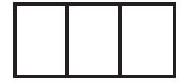
\includegraphics[max width=\textwidth, center]{2024_11_21_99eb8e6624b497a5af43g-01}

KOD\\
ZDAJĄCEGO

\section*{ZADANIA ZAMKNIĘTE}
W zadaniach 1.-25. wybierz i zaznacz jedną poprawną odpowiedź.

\section*{Zadanie 1. (0-1)}
Druga potęga liczby \(\frac{\sqrt[3]{-\frac{1}{8}} \cdot 4^{-\frac{1}{4}}}{0,25}\) jest równa:\\
A. -2\\
B. 2\\
C. 4\\
D. -4

Zadanie 2. (0-1)\\
Wiadomo, że \(\log _{5} 50=a \mathrm{i} \log _{5} 2=b\). Zatem:\\
A. \(\frac{a+b}{2}=1\)\\
B. \(\frac{a \cdot b}{2}=1\)\\
C. \(\frac{a}{b}=1\)\\
D. \(\frac{a-b}{2}=1\)

\section*{Zadanie 3. (0-1)}
W listopadzie pensja pana Jana była o \(10 \%\) większa niż w październiku. W grudniu pensja pana Jana zmalała i wynosiła o \(40 \%\) mniej niż w październiku. Średnia arytmetyczna pensji pana Jana w październiku, listopadzie i grudniu była:\\
A. o \(10 \%\) mniejsza niż w październiku\\
B. o \(15 \%\) mniejsza niż w październiku\\
C. o \(20 \%\) mniejsza niż w październiku\\
D. o 5\% większa niż w październiku

\section*{Zadanie 4. (0-1)}
Zbiór rozwiązań nierówności \((x-2)(2+x)<0\) to:\\
A. \((-\infty,-2) \cup(2,+\infty)\)\\
B. \((-\infty, 4)\)\\
C. \((-4,4)\)\\
D. \((-2,2)\)

\section*{Zadanie 5. (0-1)}
Równanie \(\frac{-3\left(9-x^{2}\right)(x+3)}{x(x+3)}=0\) :\\
A. nie ma rozwiązania\\
B. ma jedno rozwiązanie\\
C. ma dwa rozwiązania\\
D. ma trzy rozwiązania

\section*{Zadanie 6. (0-1)}
Liczba \(a\) spełniająca warunek \(\frac{2+\sqrt{3}}{a+1}=\frac{1}{2-\sqrt{3}}\) jest równa:\\
A. -3\\
B. -2\\
C. 0\\
D. 2

\section*{BRUDNOPIS (nie podlega ocenie)}
\begin{center}

\includegraphics[max width=\textwidth]{2024_11_21_99eb8e6624b497a5af43g-03}
\end{center}

\section*{Zadanie 7. (0-1)}
Układ równań \(\left\{\begin{array}{l}y=(m+2) x+2 m \\ (2 m-1) x-m=y\end{array}\right.\) opisuje w układzie współrzędnych na płaszczyźnie dwie proste równoległe. Zatem liczba \(m\) jest równa:\\
A. 0\\
B. \(-\frac{1}{3}\)\\
C. 3\\
D. \(\frac{1}{2}\)

Zadanie 8. (0-1)\\
Suma pierwiastków równania \((x-2)(x+1)(x-3)=0\) jest równa:\\
A. -6\\
B. -4\\
C. 0\\
D. 4

\section*{Zadanie 9. (0-1)}
Na rysunku przedstawiono wykres funkcji \(f\).\\
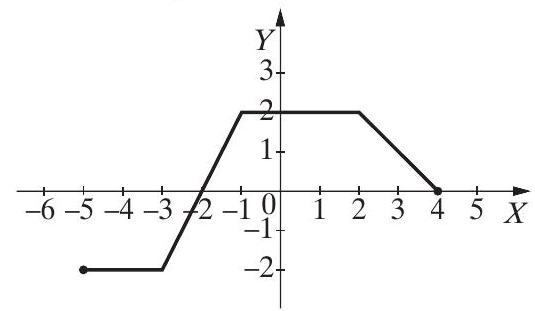
\includegraphics[max width=\textwidth, center]{2024_11_21_99eb8e6624b497a5af43g-04}

Najmniejszą wartością funkcji \(g(x)=f(-x)\) w przedziale \(\langle-4,-1\rangle\) jest liczba:\\
A. -2\\
B. -1\\
C. 0\\
D. 2

\section*{Zadanie 10. (0-1)}
Dwusieczna kąta, pod którym przecinają się proste \(y=x-1\) i \(y=-x+1\), przechodzi przez punkt:\\
A. \(P=(0,1)\)\\
B. \(P=(-1,-1)\)\\
C. \(P=(-1,1)\)\\
D. \(P=(1,0)\)

\section*{Zadanie 11. (0-1)}
W tabeli podano wartości funkcji liniowej \(f(x)=a x+b\) dla wybranych trzech elementów należących do dziedziny funkcji.

\begin{center}
\begin{tabular}{|c|c|c|c|}
\hline
\(x\) & -1 & 0 & 1 \\
\hline
\(f(x)\) & -6 & -4 & -2 \\
\hline
\end{tabular}
\end{center}

Zatem:\\
A. \(f(2)=-8\)\\
B. \(f(2)=-6\)\\
C. \(f(2)=0\)\\
D. \(f(2)=8\)

\section*{Zadanie 12. (0-1)}
Funkcja liniowa \(f\) jest określona wzorem \(f(x)=a x+b\) dla \(b=-3\) oraz \(a b<0\). Wynika z tego, że funkcja \(f\) :\\
A. jest rosnaca\\
B. jest malejąca\\
C. jest stała\\
D. nie jest ani rosnąca, ani malejąca

\section*{BRUDNOPIS (nie podlega ocenie)}
\begin{center}

\includegraphics[max width=\textwidth]{2024_11_21_99eb8e6624b497a5af43g-05}
\end{center}

\section*{Zadanie 13. (0-1)}
Dziedziną funkcji \(f\) określonej wzorem \(f(x)=(x-1)^{2}+2\) jest zbiór \(\langle-2,+\infty)\). Zbiorem wartości tej funkcji jest:\\
A. \((-\infty, 2\rangle\)\\
B. \(\langle 2,+\infty)\)\\
C. \(\langle 11,+\infty)\)\\
D. \(\langle 1,2\rangle\)

\section*{Zadanie 14. (0-1)}
Funkcja \(g\) jest opisana wzorem \(g(x)=3^{x-1}+1\). Miejscem zerowym funkcji \(h(x)=g(x+1)-4\) jest liczba:\\
A. -1\\
B. 0\\
C. 1\\
D. 3

\section*{Zadanie 15. (0-1)}
Ile liczb całkowitych należy do zbioru rozwiązań nierówności \(x-1 \leq \frac{x(x-1)-x^{2}}{2} \leq 1\) ?\\
A. 0\\
B. 1\\
C. 2\\
D. 3

\section*{Zadanie 16. (0-1)}
Suma wszystkich liczb naturalnych dodatnich podzielnych przez 5 i mniejszych od 400 jest równa:\\
A. 15800\\
B. 16000\\
C. 16040\\
D. 31600

\section*{Zadanie 17. (0-1)}
Dany jest ciąg arytmetyczny \(\left(a_{n}\right)\) określony dla \(n \geq 1\) i taki, że \(a_{1}+a_{2}+a_{3}=18\). Wtedy:\\
A. \(a_{2}=12\)\\
B. \(a_{2}=-3\)\\
C. \(a_{2}=6\)\\
D. \(a_{2}=4\)

\section*{Zadanie 18. (0-1)}
Ciąg \(\left(a_{n}\right)\) jest określony wzorem \(a_{n}=\sqrt{n-2}\) dla \(n \geq 2\). Ile wyrazów tego ciągu jest mniejszych od 2?\\
A. 2\\
B. 4\\
C. 5\\
D. nieskończenie wiele

Zadanie 19. (0-1)\\
Ciąg \((a, 2, c)\) jest geometryczny. Iloczyn wyrazów tego ciągu jest równy:\\
A. 8\\
B. 27\\
C. 64\\
D. 120

\section*{Zadanie 20. (0-1)}
W trójkącie prostokątnym kąty ostre mają miary \(\alpha, \beta\), przeciwprostokątna ma długość 13 , a \(\sin \alpha+\sin \beta=\frac{17}{13} \mathrm{i} \sin \alpha-\sin \beta=\frac{7}{13}\). Wynika z tego, że:\\
A. \(\operatorname{tg} \alpha=\frac{5}{12}\)\\
B. \(\operatorname{tg} \alpha=\frac{12}{13}\)\\
C. \(\operatorname{tg} \alpha=\frac{10}{13}\)\\
D. \(\operatorname{tg} \alpha=\frac{12}{5}\)

\section*{BRUDNOPIS (nie podlega ocenie)}
\begin{center}

\includegraphics[max width=\textwidth]{2024_11_21_99eb8e6624b497a5af43g-07}
\end{center}

\section*{Zadanie 21. (0-1)}
Kąt \(\alpha\) jest kątem ostrym takim, że \(\sin ^{2} \alpha-\cos ^{2} \alpha=\frac{1}{2}\). Zatem:\\
A. \(0^{\circ}<\alpha<20^{\circ}\)\\
B. \(21^{\circ}<\alpha<50^{\circ}\)\\
C. \(51^{\circ}<\alpha<70^{\circ}\)\\
D. \(71^{\circ}<\alpha<90^{\circ}\)

\section*{Zadanie 22. (0-1)}
Punkty \(G\) i \(H\) są środkami okręgów. Punkt \(E\) leży na okręgu o środku w punkcie \(G\), punkt \(F\) leży na okręgu o środku w punkcie \(H\) oraz \(|G H|=3 \mathrm{i}|E F|=8\) (patrz rysunek).\\
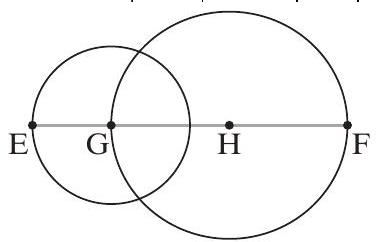
\includegraphics[max width=\textwidth, center]{2024_11_21_99eb8e6624b497a5af43g-08}

Wtedy pole koła ograniczonego okręgiem o środku w punkcie \(H\) jest większe od pola koła ograniczonego okręgiem o środku w punkcie \(G\) o:\\
A. \(25 \pi\)\\
B. \(9 \pi\)\\
C. \(14 \pi\)\\
D. \(5 \pi\)

\section*{Zadanie 23. (0-1)}
Przekątna \(A C\) dzieli trapez \(A B C D\) na dwa trójkąty prostokątne równoramienne oraz \(|\varangle B A D|=|\varangle A D C|=90^{\circ}\). Najkrótszy bok trapezu ma długość \(a\). Zatem najdłuższy bok ma długość:\\
A. \(a \sqrt{2}\)\\
B. \(2 a\)\\
C. \(a+\sqrt{2}\)\\
D. \(2 \sqrt{a}\)

\section*{Zadanie 24. (0-1)}
Okrąg o promieniu 3 jest wpisany w trójkąt prostokątny. Punkt styczności dzieli przeciwprostokątną na odcinki długości 5 i 12. Obwód tego trójkąta jest równy:\\
A. 40\\
B. 34\\
C. 51\\
D. 64

\section*{Zadanie 25. (0-1)}
Punkty \(A, M, B\) są współliniowe (punkt \(M\) leży między punktami \(A\) i \(B\) ) i takie, że \(A=(-23,-9), B=(17,21)\) oraz \(|M B|=3|A M|\). Iloczyn współrzędnych punktu \(M\) jest równy:\\
A. -18\\
B. \(-14,5\)\\
C. 19,5\\
D. 11,5

\section*{BRUDNOPIS (nie podlega ocenie)}
\begin{center}

\includegraphics[max width=\textwidth]{2024_11_21_99eb8e6624b497a5af43g-09}
\end{center}

\section*{ZADANIA OTWARTE}
Rozwiązania zadań 26.-34. należy zapisać w wyznaczonych miejscach pod treścią zadania.

Zadanie 26. (0-2)\\
Rozwiąż nierówność \(x(x-1)>2(x+1)-4\).\\

\includegraphics[max width=\textwidth, center]{2024_11_21_99eb8e6624b497a5af43g-10}

Zadanie 27. (0-2)\\
Wykaż, że jeżeli \(x>y\) i \(2(x-1)(x+1)-2 y(2 x-y)=-1\), to \(x-y=\frac{\sqrt{2}}{2}\).\\

\includegraphics[max width=\textwidth, center]{2024_11_21_99eb8e6624b497a5af43g-11}

Zadanie 28. (0-2)\\
Dany jest półokrąg oparty na średnicy \(A B\). Punkt \(C\) leży na półokręgu, punkt \(D\) leży na średnicy, odcinki \(C D\) i \(A B\) są prostopadłe oraz \(|C D|=\sqrt{2}\). Punkt \(D\) dzieli średnicę na odcinki \(a, b\) (patrz rysunek). Wykaż, że \(a b=2\).\\
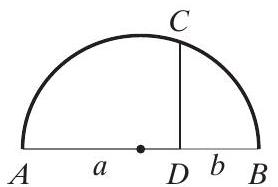
\includegraphics[max width=\textwidth, center]{2024_11_21_99eb8e6624b497a5af43g-12}\\

\includegraphics[max width=\textwidth, center]{2024_11_21_99eb8e6624b497a5af43g-12(1)}

\section*{Zadanie 29. (0-2)}
Funkcja kwadratowa ma dwa miejsca zerowe. Jednym z nich jest liczba -3. Wierzchołek paraboli, będącej wykresem tej funkcji, znajduje się w punkcie \((-1,-8)\). Wyznacz wzór tej funkcji.

\begin{center}
\begin{tabular}{|c|c|c|c|c|c|c|c|c|c|c|c|c|c|c|c|c|c|c|c|c|c|c|}
\hline
 &  &  &  &  &  &  &  &  &  &  &  &  &  &  &  &  &  &  &  &  &  &  \\
\hline
 &  &  &  &  &  &  &  &  &  &  &  &  &  &  &  &  &  &  &  &  &  &  \\
\hline
 &  &  &  &  &  &  &  &  &  &  &  &  &  &  &  &  &  &  &  &  &  &  \\
\hline
 &  &  &  &  &  &  &  &  &  &  &  &  &  &  &  &  &  &  &  &  &  &  \\
\hline
 &  &  &  &  &  &  &  &  &  &  &  &  &  &  &  &  &  &  &  &  &  &  \\
\hline
 &  &  &  &  &  &  &  &  &  &  &  &  &  &  &  &  &  &  &  &  &  &  \\
\hline
 &  &  &  &  &  &  &  &  &  &  &  &  &  &  &  &  &  &  &  &  &  &  \\
\hline
 &  &  &  &  &  &  &  &  &  &  &  &  &  &  &  &  &  &  &  &  &  &  \\
\hline
 &  &  &  &  &  &  &  &  &  &  &  &  &  &  &  &  &  &  &  &  &  &  \\
\hline
 &  &  &  &  &  &  &  &  &  &  &  &  &  &  &  &  &  &  &  &  &  &  \\
\hline
 &  &  &  &  &  &  &  &  &  &  &  &  &  &  &  &  &  &  &  &  &  &  \\
\hline
 &  &  &  &  &  &  &  &  &  &  &  &  &  &  &  &  &  &  &  &  &  &  \\
\hline
 &  &  &  &  &  &  &  &  &  &  &  &  &  &  &  &  &  &  &  &  &  &  \\
\hline
 &  &  &  &  &  &  &  &  &  &  &  &  &  &  &  &  &  &  &  &  &  &  \\
\hline
 &  &  &  &  &  &  &  &  &  &  &  &  &  &  &  &  &  &  &  &  &  &  \\
\hline
 &  &  &  &  &  &  &  &  &  &  &  &  &  &  &  &  &  &  &  &  &  &  \\
\hline
 &  &  &  &  &  &  &  &  &  &  &  &  &  &  &  &  &  &  &  &  &  &  \\
\hline
 &  &  &  &  &  &  &  &  &  &  &  &  &  &  &  &  &  &  &  &  &  &  \\
\hline
 &  &  &  &  &  &  &  &  &  &  &  &  &  &  &  &  &  &  &  &  &  &  \\
\hline
 &  &  &  &  &  &  &  &  &  &  &  &  &  &  &  &  &  &  &  &  &  &  \\
\hline
 &  &  &  &  &  &  &  &  &  &  &  &  &  &  &  &  &  &  &  &  &  &  \\
\hline
 &  &  &  &  &  &  &  &  &  &  &  &  &  &  &  &  &  &  &  &  &  &  \\
\hline
 &  &  &  &  &  &  &  &  &  &  &  &  &  &  &  &  &  &  &  &  &  &  \\
\hline
 &  &  &  &  &  &  &  &  &  &  &  &  &  &  &  &  &  &  &  &  &  &  \\
\hline
 &  &  &  &  &  &  &  &  &  &  &  &  &  &  &  &  &  &  &  &  &  &  \\
\hline
 &  &  &  &  &  &  &  &  &  &  &  &  &  &  &  &  &  &  &  &  &  &  \\
\hline
 &  &  &  &  &  &  &  &  &  &  &  &  &  &  &  &  &  &  &  &  &  &  \\
\hline
 &  &  &  &  &  &  &  &  &  &  &  &  &  &  &  &  &  &  &  &  &  &  \\
\hline
 &  &  &  &  &  &  &  &  &  &  &  &  &  &  &  &  &  &  &  &  &  &  \\
\hline
 &  &  &  &  &  &  &  &  &  &  &  &  &  &  &  &  &  &  &  &  &  &  \\
\hline
 &  &  &  &  &  &  &  &  &  &  &  &  &  &  &  &  &  &  &  &  &  &  \\
\hline
 &  &  &  &  &  &  &  &  &  &  &  &  &  &  &  &  &  &  &  &  &  &  \\
\hline
 &  &  &  &  &  &  &  &  &  &  &  &  &  &  &  &  &  &  &  &  &  &  \\
\hline
 &  &  &  &  &  &  &  &  &  &  &  &  &  &  &  &  &  &  &  &  &  &  \\
\hline
 &  &  &  &  &  &  &  &  &  &  &  &  &  &  &  &  &  &  &  &  &  &  \\
\hline
 &  &  &  &  &  &  &  &  &  &  &  &  &  &  &  &  &  &  &  &  &  &  \\
\hline
 &  &  &  &  &  &  &  &  &  &  &  &  &  &  &  &  &  &  &  &  &  &  \\
\hline
 &  &  &  &  &  &  &  &  &  &  &  &  &  &  &  &  &  &  &  &  &  &  \\
\hline
 &  &  &  &  &  &  &  &  &  &  &  &  &  &  &  &  &  &  &  &  &  &  \\
\hline
 &  &  &  &  &  &  &  &  &  &  &  &  &  &  &  &  &  &  &  &  &  &  \\
\hline
 &  &  &  &  &  &  &  &  &  &  &  &  &  &  &  &  &  &  &  &  &  &  \\
\hline
 &  &  &  &  &  &  &  &  &  &  &  &  &  &  &  &  &  &  &  &  &  &  \\
\hline
\end{tabular}
\end{center}

Zadanie 30. (0-2)\\
Prosta przechodząca przez początek układu współrzędnych ma jeden punkt wspólny z parabolą \(y=(x-1)^{2}+1\). Znajdź równanie tej prostej.\\

\includegraphics[max width=\textwidth, center]{2024_11_21_99eb8e6624b497a5af43g-14}

\section*{Zadanie 31. (0-2)}
Gdy Anka miała tyle lat, ile Danka ma teraz, to była od niej trzy razy starsza. Gdy Danka będzie miała tyle lat, ile Anka ma teraz, Anka będzie miała 42 lata. Ile lat ma obecnie każda z dziewcząt?

\begin{center}
\begin{tabular}{|c|c|c|c|c|c|c|c|c|c|c|c|c|c|c|c|c|c|c|c|c|c|c|}
\hline
 &  &  &  &  &  &  &  &  &  &  &  &  &  &  &  &  &  &  &  &  &  &  \\
\hline
 &  &  &  &  &  &  &  &  &  &  &  &  &  &  &  &  &  &  &  &  &  &  \\
\hline
 &  &  &  &  &  &  &  &  &  &  &  &  &  &  &  &  &  &  &  &  &  &  \\
\hline
 &  &  &  &  &  &  &  &  &  &  &  &  &  &  &  &  &  &  &  &  &  &  \\
\hline
 &  &  &  &  &  &  &  &  &  &  &  &  &  &  &  &  &  &  &  &  &  &  \\
\hline
 &  &  &  &  &  &  &  &  &  &  &  &  &  &  &  &  &  &  &  &  &  &  \\
\hline
 &  &  &  &  &  &  &  &  &  &  &  &  &  &  &  &  &  &  &  &  &  &  \\
\hline
 &  &  &  &  &  &  &  &  &  &  &  &  &  &  &  &  &  &  &  &  &  &  \\
\hline
 &  &  &  &  &  &  &  &  &  &  &  &  &  &  &  &  &  &  &  &  &  &  \\
\hline
 &  &  &  &  &  &  &  &  &  &  &  &  &  &  &  &  &  &  &  &  &  &  \\
\hline
 &  &  &  &  &  &  &  &  &  &  &  &  &  &  &  &  &  &  &  &  &  &  \\
\hline
 &  &  &  &  &  &  &  &  &  &  &  &  &  &  &  &  &  &  &  &  &  &  \\
\hline
 &  &  &  &  &  &  &  &  &  &  &  &  &  &  &  &  &  &  &  &  &  &  \\
\hline
 &  &  &  &  &  &  &  &  &  &  &  &  &  &  &  &  &  &  &  &  &  &  \\
\hline
 &  &  &  &  &  &  &  &  &  &  &  &  &  &  &  &  &  &  &  &  &  &  \\
\hline
 &  &  &  &  &  &  &  &  &  &  &  &  &  &  &  &  &  &  &  &  &  &  \\
\hline
 &  &  &  &  &  &  &  &  &  &  &  &  &  &  &  &  &  &  &  &  &  &  \\
\hline
 &  &  &  &  &  &  &  &  &  &  &  &  &  &  &  &  &  &  &  &  &  &  \\
\hline
 &  &  &  &  &  &  &  &  &  &  &  &  &  &  &  &  &  &  &  &  &  &  \\
\hline
 &  &  &  &  &  &  &  &  &  &  &  &  &  &  &  &  &  &  &  &  &  &  \\
\hline
 &  &  &  &  &  &  &  &  &  &  &  &  &  &  &  &  &  &  &  &  &  &  \\
\hline
 &  &  &  &  &  &  &  &  &  &  &  &  &  &  &  &  &  &  &  &  &  &  \\
\hline
 &  &  &  &  &  &  &  &  &  &  &  &  &  &  &  &  &  &  &  &  &  &  \\
\hline
 &  &  &  &  &  &  &  &  &  &  &  &  &  &  &  &  &  &  &  &  &  &  \\
\hline
 &  &  &  &  &  &  &  &  &  &  &  &  &  &  &  &  &  &  &  &  &  &  \\
\hline
 &  &  &  &  &  &  &  &  &  &  &  &  &  &  &  &  &  &  &  &  &  &  \\
\hline
 &  &  &  &  &  &  &  &  &  &  &  &  &  &  &  &  &  &  &  &  &  &  \\
\hline
 &  &  &  &  &  &  &  &  &  &  &  &  &  &  &  &  &  &  &  &  &  &  \\
\hline
 &  &  &  &  &  &  &  &  &  &  &  &  &  &  &  &  &  &  &  &  &  &  \\
\hline
 &  &  &  &  &  &  &  &  &  &  &  &  &  &  &  &  &  &  &  &  &  &  \\
\hline
 &  &  &  &  &  &  &  &  &  &  &  &  &  &  &  &  &  &  &  &  &  &  \\
\hline
 &  &  &  &  &  &  &  &  &  &  &  &  &  &  &  &  &  &  &  &  &  &  \\
\hline
 &  &  &  &  &  &  &  &  &  &  &  &  &  &  &  &  &  &  &  &  &  &  \\
\hline
 &  &  &  &  &  &  &  &  &  &  &  &  &  &  &  &  &  &  &  &  &  &  \\
\hline
 &  &  &  &  &  &  &  &  &  &  &  &  &  &  &  &  &  &  &  &  &  &  \\
\hline
 &  &  &  &  &  &  &  &  &  &  &  &  &  &  &  &  &  &  &  &  &  &  \\
\hline
 &  &  &  &  &  &  &  &  &  &  &  &  &  &  &  &  &  &  &  &  &  &  \\
\hline
 &  &  &  &  &  &  &  &  &  &  &  &  &  &  &  &  &  &  &  &  &  &  \\
\hline
 &  &  &  &  &  &  &  &  &  &  &  &  &  &  &  &  &  &  &  &  &  &  \\
\hline
 &  &  &  &  &  &  &  &  &  &  &  &  &  &  &  &  &  &  &  &  &  &  \\
\hline
 &  &  &  &  &  &  &  &  &  &  &  &  &  &  &  &  &  &  &  &  &  &  \\
\hline
 &  &  &  &  &  &  &  &  &  &  &  &  &  &  &  &  &  &  &  &  &  &  \\
\hline
\end{tabular}
\end{center}

\section*{Zadanie 32. (0-4)}
Kąt rozwarty rombu ma miarę \(2 \alpha\). Suma długości przekątnych rombu jest równa 68 oraz \(\operatorname{tg} \alpha=2,4\). Oblicz obwód rombu.\\

\includegraphics[max width=\textwidth, center]{2024_11_21_99eb8e6624b497a5af43g-16}

\section*{Zadanie 33. (0-4)}
Punkty \(A=(-4,1)\) i \(C=(-5,5)\) są wierzchołkami trójkąta równoramiennego \(A B C\), w którym \(|A C|=|B C|\). Prosta \(-x-y=0\) jest symetralną boku \(A B\). Oblicz pole tego trójkąta.\\

\includegraphics[max width=\textwidth, center]{2024_11_21_99eb8e6624b497a5af43g-17}

\section*{Zadanie 34. (0-5)}
Ciąg \((x-3, x, y)\) jest ciągiem arytmetycznym. Ciąg \((x, y, 2 y)\) jest ciągiem geometrycznym o wyrazach dodatnich. Znajdź wyrazy ciągu arytmetycznego oraz wyrazy ciągu geometrycznego.\\

\includegraphics[max width=\textwidth, center]{2024_11_21_99eb8e6624b497a5af43g-18}

\section*{BRUDNOPIS (nie podlega ocenie)}

\includegraphics[max width=\textwidth, center]{2024_11_21_99eb8e6624b497a5af43g-19}\\

\includegraphics[max width=\textwidth, center]{2024_11_21_99eb8e6624b497a5af43g-20}


\end{document}